%%%%%%%%%%%%%%%%%%%%%%%%%%%%%%%%%%%%%%%%%%%%%%%%%%%%%%%%%%%%%%%%%%%%%%%%%%%%%%%%%%%%%%%%%%%%%%%%%%%%%%%%%%%%%%%%%%%%%%%%%%%%%%%%%%%%%%%%%%%%%%%%%%%%%%%%%%%%%%%%%%%
% Written By Michael Brodskiy
% Class: Analysis of Random Phenomena
% Professor: I. Salama
%%%%%%%%%%%%%%%%%%%%%%%%%%%%%%%%%%%%%%%%%%%%%%%%%%%%%%%%%%%%%%%%%%%%%%%%%%%%%%%%%%%%%%%%%%%%%%%%%%%%%%%%%%%%%%%%%%%%%%%%%%%%%%%%%%%%%%%%%%%%%%%%%%%%%%%%%%%%%%%%%%%

\include{Includes.tex}

\title{Homework 2}
\date{\today}
\author{Michael Brodskiy\\ \small Professor: I. Salama}

\begin{document}

\maketitle

\begin{enumerate}

    \setcounter{enumi}{1}

  \item We can construct a contingency table to convey the information provided:

    \begin{center}
      \begin{tabular}[H]{|c|c|c|c|}
        \hline
        \rowcolor{black!60} \cellcolor{white} & \textcolor{white}{A} & \textcolor{white}{Not A} & \textcolor{white}{Total}\\
        \hline
        \cellcolor{black!60} \textcolor{white}{On Campus} & 40 & 160 & 200\\
        \hline
        \cellcolor{black!60} \textcolor{white}{Off Campus} & 80 & 320 & 400\\
        \hline
        \cellcolor{black!60} \textcolor{white}{Total} & 120 & 480 & 600\\
        \hline
      \end{tabular}
    \end{center}

    From here, we can calculate the probability of receiving an A as:

    $$P[A]=\frac{120}{600}=.2$$

    The probability of a student living on campus is then:

    $$P[C]=\frac{200}{600}=.33\bar{3}$$

    From the table above, we can calculate the probability of a student living on campus and getting an A:

    $$P[A\cap C]=\frac{40}{600}=.066\bar{6}$$

    From our above results we can write:

    $$P[A]P[C]=(.2)(.33\bar{3})=.066\bar{6}$$

    As such, since $P[A\cap C]=P[A]P[C]$, \underline{the two events are independent}

  \item First and foremost, we can express the probability of a router failing as $P$. From here, we can express the probability of one of the routers failing as the sum of each individual probability, less the probability that both fail. Thus, we can express this as:

    $$P[A\cup B]=2P-P^2$$

    We are given that this value equals 9\%. We can then define the probability that both fail. This can be expressed as:

    $$P[A\cap B]=P[A]P[B|A]=.2p$$

    We can solve the first equation:

    $$P^2-2P+.09=0$$
    $$P=.0461,1.9539$$

    Since we know that probability must be between 0 and 1, we get:

    $$\boxed{P=.0461}$$

    This then gives us:

    $$\boxed{P[A\cap B]=.2(.0461)=.00922}$$

    And finally, we can find the probability that no routers fail as 1 minus the probability that one of the routers fails:

    $$\boxed{P[(A\cap B)^c]=1-P[A\cup B]=.91}$$

  \item

    \begin{enumerate}

      \item We begin by calculating the total amount of options for a four and five character password. Since a digit is required, one of the characters has 10 possibilities, while the rest have $10+3+26=39$. Thus, we can write:

        $$N_4=(10)(39)^3=593190$$
        $$N_5=(10)(39)^4=23134410$$

        We then sum the two to get:

        $$N_t=N_4+N_5$$
        $$\boxed{N_t=23727600}$$

      \item We find the amount of 5-character passwords that begin with '1' as:

        $$N_1=39^4=2313441$$

        This means the probability of such a password is:

        $$P[1]=\frac{N_1}{N_5}=\frac{1}{10}$$
        $$\boxed{P[1]=.1}$$

      \item The amount of all-digit passwords may be found as:

        $$N_d=10^5+10^4=110000$$

        This gives us:

        $$P[d]=\frac{N_d}{N_t}=\frac{11000}{2313441}$$
        $$\boxed{P[d]=.004755}$$

      \item The total amount of 5-character passwords that end in a special character are:

        $$N_c=(10)(39^3)=593190$$

        This gives us:

        $$P[c]=\frac{N_c}{N_5}=\frac{1}{39}$$
        $$\boxed{P[c]=.0256}$$

    \end{enumerate}

  \item

    \begin{enumerate}

      \item Out of 25 laptops, the technician selects 5 at random, this means we have ``25 choose 5'' which can be expressed as:

        $$\left( \begin{matrix} 25\\ 5\end{matrix} \right)=\frac{25!}{5!20!}$$

        Thus, we find the total number of combinations as:

        $$\boxed{N=53130}$$

      \item We can express the number of samples containing 2 hardware issues as:

        $$N_{2H}=\left( \begin{matrix} 6\\ 2\end{matrix} \right)\left( \begin{matrix} 19\\ 3\end{matrix} \right)$$
        $$N_{2H}=\frac{6!19!}{2!4!3!16!}$$
        $$N_{2H}=14535$$

        This gives us a probability of:

        $$P[2H]=\frac{14535}{53130}$$
        $$\boxed{P[2H]=.2736}$$

      \item The probability that at least four have software issues requires the calculation of combinations with at least four software issues:

        $$N_{4+S}=\left( \begin{matrix} 6\\ 1\end{matrix} \right)\left( \begin{matrix} 19\\ 4\end{matrix} \right)\left( \begin{matrix} 6\\ 0\end{matrix} \right)\left( \begin{matrix} 19\\ 5\end{matrix} \right)$$
        $$N_{4+S}=34884$$

        We then calculate the probability:

        $$P[4+S]=\frac{34884}{53130}$$
        $$\boxed{P[4+S]=.6566}$$

      \item We calculate the total amount of possibilities with solely software and solely hardware issues:

        $$N_{5H|5S}=\left( \begin{matrix} 6\\ 5\end{matrix} \right)+\left( \begin{matrix} 19\\ 5\end{matrix} \right)$$
        $$N_{5H|5S}=11634$$

        This gives us:
        
        $$P[5H|5S]=\frac{11634}{53130}$$
        $$\boxed{P[5H|5S]=.219}$$

    \end{enumerate}

  \item

    \begin{enumerate}

      \item We begin by constructing the table. Note that all values are converted into \nth{16}s for simplicity. Given cells are highlighted in green and calculated in yellow:

    \begin{center}
      \begin{tabular}[H]{|c|c|c|c|c|}
        \hline
        \rowcolor{black!60} \cellcolor{white} & \textcolor{white}{$R_o$} & \textcolor{white}{$R_1$} & \textcolor{white}{$R_2$} & \textcolor{white}{Total}\\
        \hline
        \cellcolor{black!60} \textcolor{white}{$S$} & \cellcolor{green!50} 6/16 & \cellcolor{yellow!40} 3/16 & \cellcolor{yellow!40} 2/16 & \cellcolor{green!50} 11/16\\
        \hline
        \cellcolor{black!60} \textcolor{white}{$M$} & \cellcolor{yellow!40} 2/16 & \cellcolor{yellow!40} 1/16 & \cellcolor{green!50} 2/16 & \cellcolor{yellow!40} 5/16\\
        \hline
        \cellcolor{black!60} \textcolor{white}{Total} & \cellcolor{green!50} 8/16 & \cellcolor{green!50} 4/16 & \cellcolor{green!50} 4/16 & \cellcolor{green!50} 1\\
        \hline
      \end{tabular}
    \end{center}

      \item Per the table above, the probability is:

        $$P[R_2|S]=\frac{2}{16}\cdot\frac{16}{11}$$
        $$\boxed{P[S\cap R_2]=.1818}$$

      \item Per the table above, we can calculate this as:

        $$P[(R_o\cup R_1)|M]=\left(\frac{2}{16}+\frac{1}{16}\right)\cdot\frac{16}{5}$$
        $$\boxed{P[(R_o\cup R_1)|M]=.6}$$

      \item We can calculate this as:

        $$P[R_o|(R_o\cup R_1)]=\frac{P[R_o]}{P[R_o]+P[R_1]}$$
        $$P[R_o|(R_o\cup R_1)]=\frac{1/2}{3/4}$$
        $$\boxed{P[R_o|(R_o\cup R_1)]=.66\bar{6}}$$

    \end{enumerate}

  \item

    \begin{enumerate}

      \item We begin by writing down the given information:

        $$P[S]=.9$$
        $$P[I]=1-.9=.1$$
        $$P[C|I]=.5$$
        $$P[C|S]=.2$$
        $$P[D|(C\cap I)]=.75$$
        $$P[D|(C^c\cap S)]=.75$$
        $$P[D|(C^c\cap I)\cup (C\cap S)]=.3$$

      \item 

      \item 

      \item 

    \end{enumerate}

  \item

    \begin{enumerate}

      \item We may begin by writing down given information:

        $$P[N]=.7$$
        $$P[M]=.4$$
        $$P[N\cap M]=.1$$
        $$P[R_N|N]=.75$$
        $$P[R_M|M]=.8$$
        $$P[(R_N\cup R_M) |(N\cap M)]=.9$$

        We need to calculate the individual probabilities that a customer renews a single service or both and sum them together. Per Bayes' Theorem, we know:

        $$P[X|Y]=\frac{P[X\cap Y]}{P[Y]}$$

        Since we want to find $P[R_N\cap N]$, $P[R_M\cap M]$, and $P[(R_N\cap R_M)\cap(N\cap M)]$, we get:

        $$P[R_N\cap N]=P[N]P[R_N|N]=(.7)(.75)$$
        $$P[R_M\cap M]=P[M]P[R_M|M]=(.4)(.8)$$
        $$P[(R_N\cap R_M)\cap(N\cap M)]=P[(M\cap N)]P[(R_N\cup R_M) |(N\cap M)]=(.1)(.9)$$

        This gives us:

        $$\boxed{P[R_N\cap N]=.525}$$
        $$\boxed{P[R_M\cap M]=.32}$$
        $$\boxed{P[(R_N\cap R_M)\cap(N\cap M)]=.09}$$

        We then sum the individual probabilities to get the overall probability of renewal:

        $$\boxed{P[R_N\cup R_M\cup (R_N\cap R_M)]=.525+.32+.09=.935}$$

      \item Here, our goal is to find $P[(N\cap M)|(R_N\cup R_M)]$ and $P[(N\cup M)|(R_N\cup R_M)]$. Per Bayes Rule, we know:

        $$P[A|B]=\frac{P[B|A]P[A]}{P[B]}$$

        Applying this to the current situation, we find:

        $$P[(N\cap M)|(R_N\cup R_M)]=\frac{P[(R_N\cup R_M) |(N\cap M)]P[N\cap M]}{P[R_N\cup R_M]}$$
        $$P[(N\cap M)|(R_N\cup R_M)]=\frac{(.9)(.1)}{.935}$$
        $$\boxed{P[(N\cap M)|(R_N\cup R_M)]=.096257}$$

        We can then find the alternate probability as:

        $$P[(N\cup M)|(R_N\cup R_M)]=1-.096257$$
        $$\boxed{P[(N\cup M)|(R_N\cup R_M)]=.9037}$$

      \item This can be taken as the complement of the probability from part (a):

        $$\boxed{P[R^c]=1-.935=.065}$$

    \end{enumerate}

  \item

    \begin{enumerate}

      \item A tree diagram can be constructed as follows:

        \begin{figure}[H]
          \centering
          \tikzset{every picture/.style={line width=0.75pt}} %set default line width to 0.75pt        

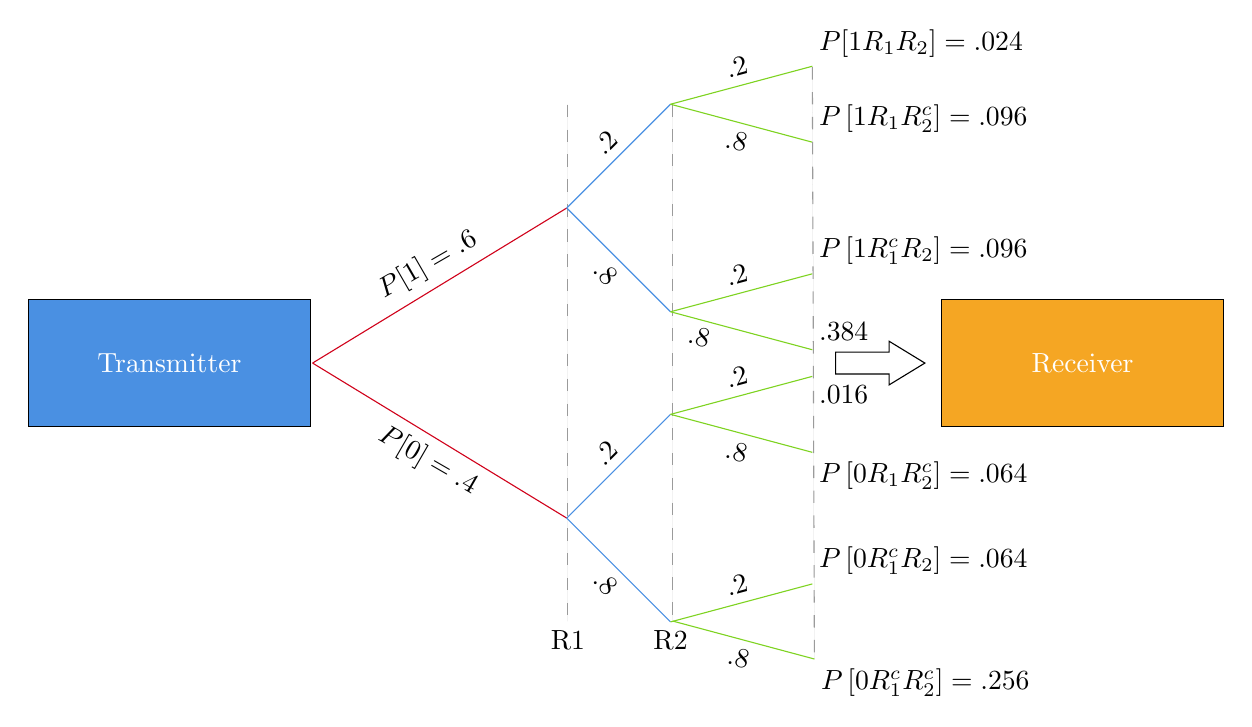
\begin{tikzpicture}[x=0.75pt,y=0.75pt,yscale=-1,xscale=1]
%uncomment if require: \path (0,375); %set diagram left start at 0, and has height of 375

%Straight Lines [id:da7733451095996544] 
\draw [color={rgb, 255:red, 208; green, 2; blue, 27 }  ,draw opacity=1 ]   (147,195.5) -- (269.47,270.21) ;
%Shape: Rectangle [id:dp6454339282474542] 
\draw  [fill={rgb, 255:red, 74; green, 144; blue, 226 }  ,fill opacity=1 ] (10,165) -- (146,165) -- (146,226) -- (10,226) -- cycle ;
%Straight Lines [id:da8481277726765063] 
\draw [color={rgb, 255:red, 155; green, 155; blue, 155 }  ,draw opacity=1 ][fill={rgb, 255:red, 155; green, 155; blue, 155 }  ,fill opacity=1 ] [dash pattern={on 4.5pt off 4.5pt}]  (270,71) -- (270,320) ;
%Straight Lines [id:da022158918268141536] 
\draw [color={rgb, 255:red, 208; green, 2; blue, 27 }  ,draw opacity=1 ]   (147,195.5) -- (269.47,120.79) ;
%Straight Lines [id:da7936419917799142] 
\draw [color={rgb, 255:red, 74; green, 144; blue, 226 }  ,draw opacity=1 ]   (269.47,270.21) -- (319.47,220.21) ;
%Straight Lines [id:da035414361338925726] 
\draw [color={rgb, 255:red, 74; green, 144; blue, 226 }  ,draw opacity=1 ]   (269.47,120.79) -- (319.47,170.79) ;
%Straight Lines [id:da6315531716142546] 
\draw [color={rgb, 255:red, 74; green, 144; blue, 226 }  ,draw opacity=1 ]   (269.47,270.21) -- (319.47,320.21) ;
%Straight Lines [id:da43044094613045636] 
\draw [color={rgb, 255:red, 74; green, 144; blue, 226 }  ,draw opacity=1 ]   (269.47,120.79) -- (319.47,70.79) ;
%Straight Lines [id:da3197820199985336] 
\draw [color={rgb, 255:red, 155; green, 155; blue, 155 }  ,draw opacity=1 ][fill={rgb, 255:red, 155; green, 155; blue, 155 }  ,fill opacity=1 ] [dash pattern={on 4.5pt off 4.5pt}]  (320.47,70.79) -- (320.47,319.79) ;
%Straight Lines [id:da3376346045191835] 
\draw [color={rgb, 255:red, 126; green, 211; blue, 33 }  ,draw opacity=1 ]   (319.47,70.79) -- (387.78,52.49) ;
%Straight Lines [id:da5341817002427772] 
\draw [color={rgb, 255:red, 126; green, 211; blue, 33 }  ,draw opacity=1 ]   (319.47,70.79) -- (387.78,89.09) ;
%Straight Lines [id:da9132861107764135] 
\draw [color={rgb, 255:red, 126; green, 211; blue, 33 }  ,draw opacity=1 ]   (319.47,170.79) -- (387.78,152.49) ;
%Straight Lines [id:da0948837605825038] 
\draw [color={rgb, 255:red, 126; green, 211; blue, 33 }  ,draw opacity=1 ]   (319.47,170.79) -- (387.78,189.09) ;
%Straight Lines [id:da5858203477238184] 
\draw [color={rgb, 255:red, 126; green, 211; blue, 33 }  ,draw opacity=1 ]   (319.47,220.21) -- (387.78,201.91) ;
%Straight Lines [id:da7551891548818732] 
\draw [color={rgb, 255:red, 126; green, 211; blue, 33 }  ,draw opacity=1 ]   (319.47,220.21) -- (387.78,238.51) ;
%Straight Lines [id:da9857178211203643] 
\draw [color={rgb, 255:red, 126; green, 211; blue, 33 }  ,draw opacity=1 ]   (319.47,320.21) -- (387.78,301.91) ;
%Straight Lines [id:da15601066335308467] 
\draw [color={rgb, 255:red, 126; green, 211; blue, 33 }  ,draw opacity=1 ]   (320.47,319.79) -- (388.78,338.09) ;
%Straight Lines [id:da8229205540347613] 
\draw [color={rgb, 255:red, 155; green, 155; blue, 155 }  ,draw opacity=1 ][fill={rgb, 255:red, 155; green, 155; blue, 155 }  ,fill opacity=1 ] [dash pattern={on 4.5pt off 4.5pt}]  (387.78,52.91) -- (388.78,338.09) ;
%Shape: Rectangle [id:dp08161365143596533] 
\draw  [fill={rgb, 255:red, 245; green, 166; blue, 35 }  ,fill opacity=1 ] (450,165) -- (586,165) -- (586,226) -- (450,226) -- cycle ;
%Right Arrow [id:dp6874336891615508] 
\draw   (399,190.25) -- (424.8,190.25) -- (424.8,185) -- (442,195.5) -- (424.8,206) -- (424.8,200.75) -- (399,200.75) -- cycle ;

% Text Node
\draw (78,195.5) node  [color={rgb, 255:red, 255; green, 255; blue, 255 }  ,opacity=1 ] [align=left] {Transmitter};
% Text Node
\draw (206.54,155.2) node [anchor=south] [inner sep=0.75pt]  [rotate=-330]  {$P[ 1] =.6$};
% Text Node
\draw (206.54,235.8) node [anchor=north] [inner sep=0.75pt]  [rotate=-30]  {$P[ 0] =.4$};
% Text Node
\draw (270,323) node [anchor=north] [inner sep=0.75pt]   [align=left] {R1};
% Text Node
\draw (292.07,93.39) node [anchor=south] [inner sep=0.75pt]  [rotate=-315]  {$.2$};
% Text Node
\draw (292.07,148.19) node [anchor=north] [inner sep=0.75pt]  [rotate=-45]  {$.8$};
% Text Node
\draw (292.07,297.61) node [anchor=north] [inner sep=0.75pt]  [rotate=-45]  {$.8$};
% Text Node
\draw (292.07,242.81) node [anchor=south] [inner sep=0.75pt]  [rotate=-315]  {$.2$};
% Text Node
\draw (319.47,323.21) node [anchor=north] [inner sep=0.75pt]   [align=left] {R2};
% Text Node
\draw (352.75,58.35) node [anchor=south] [inner sep=0.75pt]  [rotate=-345]  {$.2$};
% Text Node
\draw (352.75,83.22) node [anchor=north] [inner sep=0.75pt]  [rotate=-15]  {$.8$};
% Text Node
\draw (334.75,177.22) node [anchor=north] [inner sep=0.75pt]  [rotate=-15]  {$.8$};
% Text Node
\draw (352.75,232.65) node [anchor=north] [inner sep=0.75pt]  [rotate=-15]  {$.8$};
% Text Node
\draw (353.75,332.22) node [anchor=north] [inner sep=0.75pt]  [rotate=-15]  {$.8$};
% Text Node
\draw (352.75,158.35) node [anchor=south] [inner sep=0.75pt]  [rotate=-345]  {$.2$};
% Text Node
\draw (352.75,207.78) node [anchor=south] [inner sep=0.75pt]  [rotate=-345]  {$.2$};
% Text Node
\draw (352.75,307.78) node [anchor=south] [inner sep=0.75pt]  [rotate=-345]  {$.2$};
% Text Node
\draw (518,195.5) node  [color={rgb, 255:red, 255; green, 255; blue, 255 }  ,opacity=1 ] [align=left] {Receiver};
% Text Node
\draw (389.78,49.51) node [anchor=south west] [inner sep=0.75pt]    {$P[ 1R_{1} R_{2}] =.024$};
% Text Node
\draw (389.78,149.09) node [anchor=south west] [inner sep=0.75pt]    {$P\left[ 1R_{1}^{c} R_{2}\right] =.096$};
% Text Node
\draw (389.78,85.69) node [anchor=south west] [inner sep=0.75pt]    {$P\left[ 1R_{1} R_{2}^{c}\right] =.096$};
% Text Node
\draw (389.78,185.69) node [anchor=south west] [inner sep=0.75pt]    {$.384$};
% Text Node
\draw (389.78,205.31) node [anchor=north west][inner sep=0.75pt]    {$.016$};
% Text Node
\draw (389.78,241.91) node [anchor=north west][inner sep=0.75pt]    {$P\left[ 0R_{1} R_{2}^{c}\right] =.064$};
% Text Node
\draw (389.78,298.51) node [anchor=south west] [inner sep=0.75pt]    {$P\left[ 0R_{1}^{c} R_{2}\right] =.064$};
% Text Node
\draw (390.78,341.49) node [anchor=north west][inner sep=0.75pt]    {$P\left[ 0R_{1}^{c} R_{2}^{c}\right] =.256$};


\end{tikzpicture}

          \caption{Tree Diagram for Routing Problem}
          \label{fig:1}
        \end{figure}

      \item This would be represented by the sequence $1R_1^cR_2^c$. As the tree diagram suggests, we see:

        $$\boxed{P[1R_1^cR_2^c]=.384}$$

      \item Given that a '1' is sent by the transmitter, a '1' is received by the receiver in the sequences: $1R_1^cR_2^c$ and $1R_1R_2$. We sum the probabilities to get:

        $$\boxed{P[1_R|1_T]=.384+.024=.408}$$

      \item We now factor in receiving a '1' when a '0' is transmitted:

        $$\boxed{P[1_R]=P[1_R|1_T] + 2(.064)=.536}$$

      \item We can take the '1' sent '1' received case from part (c) and divide it by the '1' received general case to get:

        $$\boxed{P[1_T|1_R]=.7612}$$

    \end{enumerate}

  \item

    \begin{itemize}

      \item Expected quantity of days over a week case

        For this case, we simply multiply each probability (as each one represents the ``status per day'' probability) by the quantity of days in a week, or 7. This gets us:

        $$N_E=\frac{63}{20}$$
        $$\boxed{N_E=3.15[\text{days per week}]}$$

        $$N_M=\frac{21}{20}$$
        $$\boxed{N_M=1.05[\text{days per week}]}$$

        $$N_C=\frac{56}{20}$$
        $$\boxed{N_C=2.8[\text{days per week}]}$$

      \item Probability of 4 efficient, 1 moderate, and 2 congested days in a week

        We can represent this as a sequence of probabilities of each state per day. This gives us:

        $$P[4E \cap 1M\cap 2C]=\frac{7!}{4!2!1!}\left( \frac{9}{20} \right)^4\left( \frac{3}{20} \right)\left( \frac{8}{20} \right)^2$$
        $$\boxed{P[4E \cap 1M\cap 2C]=.1033}$$

      \item Probability of equivalent days congested and efficient

        There are four cases where this is true: a 3/3, 2/2, 1/1, and 0/0 split. We sum the probability of each individual state to get:

        $$P[E=C]=\sum_{i=0}^3\frac{7!}{(i!)^2(7-2i)!}\left(  \frac{9}{20}\right)^i\left( \frac{8}{20} \right)^i\left( \frac{3}{20} \right)^{7-2i}$$
        $$\boxed{P[E=C]=.146}$$

    \end{itemize}

\end{enumerate}

\end{document}

